\documentclass[
	12pt,
	]{article}
		\usepackage{xcolor}
			\usepackage[dvipsnames]{xcolor}
			\usepackage[many]{tcolorbox}
		\usepackage{changepage}
		\usepackage{titlesec}
		\usepackage{caption}
		\usepackage{mdframed, longtable}
		\usepackage{mathtools, amssymb, amsfonts, amsthm, bm,amsmath} 
		\usepackage{array, tabularx, booktabs}
		\usepackage{graphicx,wrapfig, float, caption}
		\usepackage{tikz,physics,cancel, siunitx, xfrac}
		\usepackage{graphics, fancyhdr}
		\usepackage{lipsum}
		\usepackage{xparse}
		\usepackage{thmtools}
		\usepackage{mathrsfs}
		\usepackage{undertilde}
		\usepackage{tikz}
		\usepackage{fullpage,enumitem}
		\usepackage[labelfont=bf]{caption}
		\usepackage{hyperref}
	\newcommand{\td}{\text{dim}}
	\newcommand{\tvw}{T : V\xrightarrow{} W }
	\newcommand{\ttt}{\widetilde{T}}
	\newcommand{\ex}{\textbf{Example}}
	\newcommand{\aR}{\alpha \in \mathbb{R}}
	\newcommand{\abR}{\alpha \beta \in \mathbb{R}}
	\newcommand{\un}{u_1 , u_2 , \dots , n}
	\newcommand{\an}{\alpha_1, \alpha_2, \dots, \alpha_2 }
	\newcommand{\sS}{\text{Span}(\mathcal{S})}
	\newcommand{\sSt}{($\mathcal{S}$)}
	\newcommand{\la}{\langle}
	\newcommand{\ra}{\rangle}
	\newcommand{\Rn}{\mathbb{R}^{n}}
	\newcommand{\R}{\mathbb{R}}
	\newcommand{\Rm}{\mathbb{R}^{m}}
	\usepackage{fullpage, fancyhdr}
	\newcommand{\La}{\mathcal{L}}
	\newcommand{\ep}{\epsilon}
	\newcommand{\de}{\delta}
	\usepackage[math]{cellspace}
		\setlength{\cellspacetoplimit}{3pt}
		\setlength{\cellspacebottomlimit}{3pt}


	\usepackage{mathtools}
	\newcommand{\vectorproj}[2][]{\textit{proj}_{\vect{#1}}\vect{#2}}
	\newcommand{\vect}{\mathbf}
	\newcommand{\uuuu}{\sum_{i=1}^{n}\frac{<u,u_i}{<u_i,u_i>} u_i}
	\newcommand{\B}{\mathcal{B}}
	\newcommand{\Ss}{\mathcal{S}}
	
	\newtheorem{theorem}{Theorem}[section]
	\theoremstyle{definition}
	\newtheorem{corollary}{Corollary}[theorem]
	\theoremstyle{definition}
	\newtheorem{lemma}[theorem]{Lemma}
	\theoremstyle{definition}
	\newtheorem{definition}{Definition}[section]
	\theoremstyle{definition}
	\newtheorem{Proposition}{Proposition}[section]
	\theoremstyle{definition}
	\newtheorem*{example}{Example}
	\theoremstyle{example}
	\newtheorem*{note}{Note}
	\theoremstyle{note}
	\newtheorem*{remark}{Remark}
	\theoremstyle{remark}
	\newtheorem*{example2}{External Example}
	\theoremstyle{example}
	
	\title{PHYS 350 Assignment 1}
	\titleformat*{\section}{\LARGE\normalfont\fontsize{12}{12}\bfseries}
	\titleformat*{\subsection}{\Large\normalfont\fontsize{10}{15}\bfseries}
	\author{Mihail Anghelici 260928404 }
	\date{\today}
	
	\relpenalty=9999
			\binoppenalty=9999
		
			\renewcommand{\sectionmark}[1]{%
			\markboth{\thesection\quad #1}{}}
			
			\fancypagestyle{plain}{%
			  \fancyhf{}
			  \fancyhead[L]{\rule[0pt]{0pt}{0pt} Assignment 1 } 
			  \fancyhead[R]{\small Mihail Anghelici $260928404$} 
			  \fancyfoot[C]{-- \thepage\ --}
			  \renewcommand{\headrulewidth}{0.4pt}}
			\pagestyle{plain}
			\setlength{\headsep}{1cm}
	\captionsetup{margin =1cm}
	\begin{document}
	\maketitle
		\section*{Question 1 }
			\subsection*{a) }
			To show this relationship we will use two lemmas :
			\begin{itemize}
				\item $\de_{ii} = \sum_{i=1}^{3}\de_{ii} = 1+1+1 = 3.$
				\item $\de_{ij}\de_{jk} = \de_{ik}.$
			\end{itemize}
				\begin{align*}
					\epsilon_{ijk}\epsilon_{klm} &= \de_{il}\de_{jm}-\de_{im}\de_{jl} = \begin{vmatrix}
						\de_{ik} & \de_{il} &\de_{im} \\
						\de_{jk} & \de_{jl} &\de_{jm} \\
						\de_{kk} & \de_{kl} &\de_{km}
					\end{vmatrix} \\
					&= 3(\de_{il}\de_{jm} -\de_{im}\de_{jl})-\de_{jk}(\de_{il}\de_{km}-\de_{im}\de_{kl}) + \de_{ik}(\de_{jl}\de_{km} - \de_{jm}\de_{kl}) \\
					&=3\de_{il}\de_{jm}-3\de_{im}\de_{jl} -\de_{jm}\de_{il}+\de_{jl}\de_{im}+\de_{im}\de_{jl}-\de_{il}\de_{jm}\\
					&= \de_{il}\de_{jm}-\de_{im}\de_{jl}.
				\end{align*}
			\subsection*{b) }
				\begin{align*}
					\vec{A}\cross (\vec{B}\cross \vec{C}) &= \ep_{ijk}A_{j}(\ep_{klm}B_{l}C_{m})\\
					&=\ep_{ijk}\ep_{klm}A_{j}B_{l}C_{m} \\
					&=(\de_{il}\de_{jm}-\de_{im}\de_{jl})A_{j}B_{l}C_{m}\\
					&=\de_{il}\de_{jm}(A_{j}B_{l}C_{m}) - \de_{im}\de_{jl}(A_{j}B_{l}C_{m})\\
					&=A_{j}B_{i}C_{j} - A_{j}B_{j}C_{i} \\
					&= \vec{B}(\vec{A}\cdot\vec{C}) - \vec{C}(\vec{A}\cdot \vec{B}).
				\end{align*}
			\section*{Question 2}
				\subsection*{a) }
					\begin{figure}[H]
				   		 	   		 	\centering
				   		 	   		 	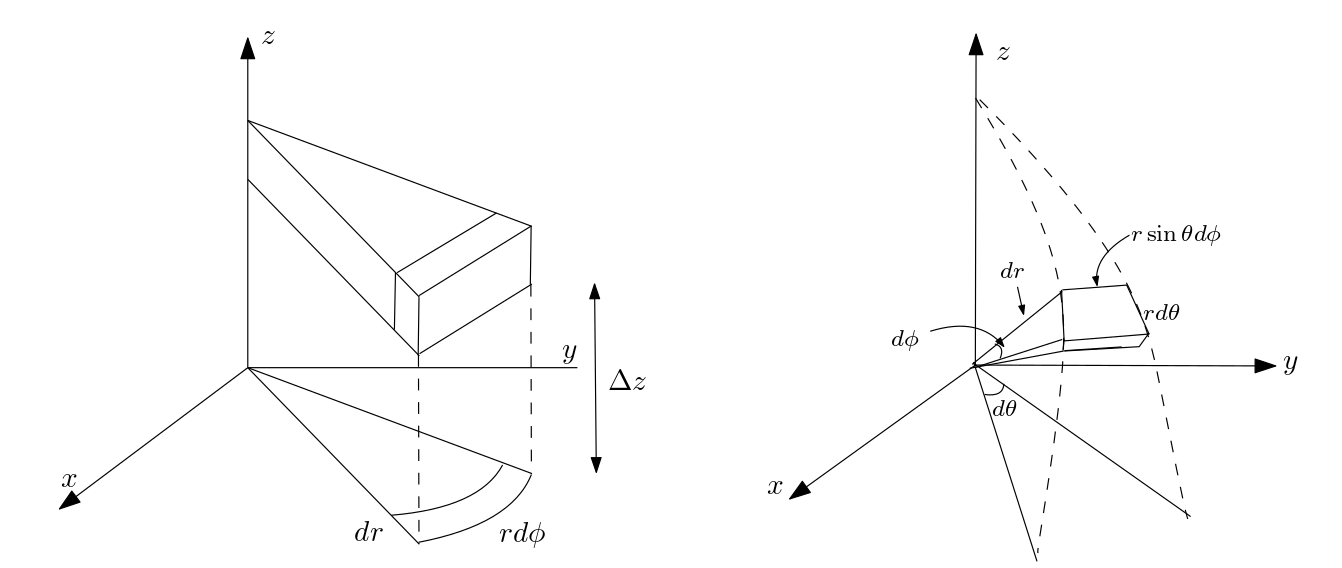
\includegraphics[width=1.0\linewidth]{PHYS350_Ass1_Cyl_Spher.png}
				   		 	   		 	\captionsetup{margin=1cm, justification=raggedright}\caption{\textbf{(a)}Infinitesimal slab of a cylinder. \textbf{(b)} Infinitesimal slab of a sphere}
		   		 	 \end{figure}
		   		 In the $r$ direction we have 
		   		 \begin{itemize}
		   		 	\item $f_{r} rd\phi dz$
		   		 	\item $f_{r+\Delta r}rd\phi dz = (f_{r}r + dr \pdv{(f_{r} r)}{\partial r}) d\phi dz $
		   		 \end{itemize}
		   		 We note that $r$ is an implicit variable therefore it is embedded in the argument of $\partial (f_{r} r)$. The net force is then 
		   		 $$ \text{Net } = (f_{r}r + dr \pdv{(f_{r} r)}{r}) d\phi dz - f_{r} rd\phi dz = \pdv{(f_{r} r)}{r} dr d\phi dz.$$
		   		 In the $\phi$ direction :
		   		 \begin{itemize}
		   		 	\item $f_{\phi}dr dz$
		   		 	\item $f_{\phi+ \Delta \phi} dr dz = (f_{\phi}+d\phi \pdv{f_{\phi}}{\phi})dr dz$
		   		 \end{itemize}
		   		 Net force is then 
		   		 $$ \text{Net } = (f_{\phi}+d\phi \pdv{f_{\phi}}{\phi})dr dz- f_{\phi}dr dz = \pdv{f_{\phi}}{\phi}dr d\phi dz.$$
		   		 In the $z$ direction : 
		   		 \begin{itemize}
		   		 	\item $f_{z} r dr \phi $
		   		 	\item $f_{z+\Delta z} r dr d\phi = (f_{z}+dz \pdv{f_{z}}{z})r dr d\phi$
		   		 \end{itemize}
		   		 The net force is then 
		   		 $$ \text{Net } = (f_{z}+dz \pdv{f_{z}}{z})r dr d\phi - f_{z} r dr \phi = \pdv{f_{z}}{z} r dr d\phi dz.$$
		   		 Finally adding up all the results and dividing by $r$ to account for the extra $r$ in the $z$ direction we have 
		   		 $$ \vec{\nabla} \cdot \vec{f} = \left(\left(\frac{1}{r}\right)\pdv{f_{r}r}{r} + \left(\frac{1}{r}\right) \pdv{f_{\phi}}{\phi} + \pdv{f_{z}}{z}\right)dr d\phi dz.$$
		   		 
		   		 \subsection*{b) }
		   		 
		   		 \noindent We proceed similarly for the spherical coordinates. First, in the $r$ direction 
		   		 \begin{itemize}
		   		 	\item $f_{r}r^{2}\sin \theta d \phi d\theta$ 
		   		 	\item $f_{r+ \Delta r} r^{2}\sin\theta d\phi d\theta  = (f_{r}r^{2}+dr\pdv{f_{r}r^{2}}{r}) d\phi d\theta$
		   		 \end{itemize}
		   		 We proceed similarly as in the $r$ direction of Question $2 \text{a}$ in which we embedded the $r$ value in the argument of the partial derivative , since it's an implicit value. The net force is then 
		   		 $$ \text{Net } = (f_{r}r^{2}+dr\pdv{f_{r}r^{2}}{r}) d\phi d\theta - f_{r}r^{2}\sin \theta d \phi d\theta = \pdv{f_{r}r^{2}}{r} dr d\phi d\theta.$$
		   		 
		   		 In the $\theta $ direction :
		   		 \begin{itemize}
		   		 	\item $f_{\theta} r\sin \theta d\phi dr $
		   		 	\item $f_{\theta + \Delta \theta} r\sin \theta d\phi dr = (f_{r}\sin\theta + d\theta \pdv{f_{\theta }\sin\theta}{\theta}) r d\phi dr$
		   		 \end{itemize}
		   		 The net force is then 
		   		 $$ \text{Net } = (f_{r}\sin\theta + d\theta \pdv{f_{\theta }\sin\theta}{\theta}) r d\phi dr - f_{\theta} r\sin \theta d\phi dr  = \pdv{f_{\theta}\sin\theta}{\theta} r d\theta dr d\phi .$$
		   		 
		   		 In the $\phi $ direction : 
		   		 \begin{itemize}
		   		 	\item $f_{\phi} r dr d\theta$ 
		   		 	\item $f_{\phi + \Delta \phi}r dr d\theta = (f_{\phi} + d\phi \pdv{f_{\phi}}{\phi})r drd\theta$
		   		 \end{itemize}
		   		 The net force is 
		   		 $$ \text{Net } = (f_{\phi} + d\phi \pdv{f_{\phi}}{\phi})r drd\theta - f_{\phi} r dr d\theta = \pdv{f_{\phi}}{\phi} r dr d\theta d\phi.$$
		   		 
		   		 \noindent Adding up everything and diving by $r^{2}\sin\theta$ to clean up the expression and match the arguments with the divided elements we obtain 
		   		 \begin{equation} 
		   		  \vec{\nabla}\cdot \vec{f} = \left(\left(\frac{1}{r^{2}}\right)\pdv{(f_{r}r^{2})}{r} + \left(\frac{1}{r \sin\theta}\right) \pdv{f_{\theta}\sin \theta}{\theta} + \left(\frac{1}{r\sin \theta}\right) \pdv{f_{\phi}}{\phi}\right) dr d\theta d\phi.
		   		  \end{equation}
			\section*{Question 3 }
				To solve this, we use the result found previously $(1)$. 
				\begin{align*}
					\text{div}F = \vec{\nabla} \cdot \vec{F} &= \frac{1}{r^{2}} \frac{\partial}{\partial r} (r^{2} F_{r}) \\
					&= \frac{1}{r^{2}} \frac{\partial}{\partial r} \left(r^{2}\frac{1}{r^{2+\ep}}\right)\\ 
					&= \frac{1}{r^{2}} \frac{\partial}{\partial r} (r^{-\ep}) \\
					&= \left(\frac{-\ep }{r^{2}}\right) \frac{1}{r^{\ep +1}} = -\frac{\ep}{r^{\ep + 3}} \quad, \text{for } \ r\in \mathbb{R} \setminus \{0\}.
				\end{align*} 	   	
			\section*{Question 4}
				$q_{1} = q_{2}\equiv q$ and $m_{p} = m_{p} \equiv m$ In (MKS),
				\begin{gather*}
					\frac{F_{e}}{F_{g}} = \frac{\frac{kq^{2}}{r^{2}}}{\frac{Gm^{2}}{r^{2}}} = \frac{kq^{2}}{Gm^{2}}
					= \frac{(8.987 \cross 10^{9})(1.602 \cross 10^{-19})^{2}}{(1,672\cross 10^{-27})^{2}(6.67\cross 10^{-11})} \frac{\si{\newton}}{\si{\newton}} \approx  1.237 \cross 10^{36}.
				\end{gather*} 
			It is to be noted that the choice of the unit system (MKS, CGS, English) does not matter in this context since the fraction is dimensionless. 
			
			\section*{Question 5}
				\subsection*{a) }
					We find the minimal $\delta t$ by setting the uncertainty principle equal. 
					$$ \delta t = \frac{\hbar}{2 m c^{2}}.$$
					The maximal rest mass is found in the same way while setting $c\delta t = d = 100 000 \ \text{ly}$.
					$$ \delta E \delta t \le \frac{\hbar}{2} \xrightarrow{} d= c\delta t \implies d = \frac{\hbar }{2mc} \implies m = \frac{\hbar }{200 000 \ \text{ly c}}.$$	
				\subsection*{b) }
					If the photon doesn't have a mass then $E \sim \frac{1}{4\pi \ep_{0}r^{2}}$. Alternatively, if the photon does have a mass, then the electric field has a bonus decay $E \sim \frac{q}{4\pi ep_{0}r^{2}}e^{-r/r_{0}}$.
					
					\noindent We set $r_{0} = 100 000 \ \text{ly} = 100 000(9.46\cross 10^{15}) \ \si{\meter}$ and set $r = 10 000 \ \si{\kilo\meter} = 10^{7} \ \si{\meter}$. We take the fraction of the two electric fields 
					$$ \frac{\frac{q}{4\pi ep_{0}r^{2}}e^{-r/r_{0}}}{\frac{1}{4\pi \ep_{0}r^{2}}}= e^{-r/r_{0}} = \exp{-\frac{10^{7} \ \si{\meter}}{100 000(9.46\cross 10^{15}) \ \si{\meter}}} = e^{-1.05\cross 10^{-14}} \approx 0.999.$$ 
				\section*{Bonus} 
					GitHub username : PhysicsKush 
					
					URL to the project code : 
					
					\centering{
						 \url{https://github.com/physicskush/PHYS350_Ass1/blob/master/PHYS350_Ass1_bonus.ipynb}
					}
	\end{document}